\chapter{Switch}

\section{Operation}

\subsection{Switch boot sequence}

After a Cisco switch is powered on, it goes through the following boot sequence:

\begin{enumerate}
\item The switch loads a power-on self-test (POST) program stored in ROM.

\item Boot loader software is loaded.

\item The boot loader initializes the CPU registers.

\item The boot loader initializes the flash file system.

\item The boot loader loads IOS image into RAM and gives control of the switch to the IOS.

\item The IOS initializes the startup-config file, which is stored in NVRAM.
\end{enumerate}

The boot loader software finds the Cisco IOS image using \emph{Boot environment variables}. If this variable is not set, the switch attempts to load and execute the first executable file it finds. Use the command \code{show boot} to see content of the the variable and what the current IOS boot file is set to.

\begin{sexylisting}{Setting boot environment variable}
boot system flash:/c2960-lanbasek9-mz.150-2.SE/c2960-lanbasek9-mz.150-2.SE.bin
\end{sexylisting}

\subsection{MAC address table}

A Layer 2 Ethernet switch uses MAC addresses to make forwarding decisions. It consults a MAC address table to make a forwarding decision for each frame. By default, most Ethernet switches keep an entry in the MAC address table for 5 minutes.

\paragraph{Learning MAC Address:} The switch dynamically builds the MAC address table by examining the source MAC address of the frames received on a port. Every frame that enters a switch is checked for new information to learn. If the source MAC address does not exist, it is added to the table along with the incoming port number. If the source MAC address does exist, the switch updates the refresh timer for that entry.  If the source MAC address does exist in the table but on a different port, the switch treats this as a new entry.

\paragraph{Forwarding MAC Address:} Next, if the destination MAC address is a unicast address, the switch will look for a match between the destination MAC address of the frame and an entry in its MAC address table. If the destination MAC address is in the table, it will forward the frame out the specified port. If the destination MAC address is not in the table, the switch will forward the frame out all ports except the incoming port. If the destination MAC address is a broadcast or a multicast, the frame is also flooded out all ports except the incoming port.\\

A switch can have multiple MAC addresses associated with a single port. This is common when the switch is connected to another switch.

\subsection{Frame forwarding method}

A switch makes a decision on frame forwarding based on two criteria: \textbf{Ingress port} and \textbf{Destination address}. Switches use one of the following forwarding methods:  Store-and-forward switching and Cut-through switching.

\paragraph{Store-and-forward switching:} has two primary characteristics that distinguish it from cut-through: \textbf{error checking} and \textbf{automatic buffering}. When the switch receives the frame, it stores the data in buffers until the complete frame has been received. In this process, the switch also performs an error checking using the CRC trailer portion of the Ethernet frame. When an error is detected in a frame, the switch discards the frame. Discarding frames with errors reduces the amount of bandwidth consumed by corrupt data. Store-and-forward switching is required for Quality of Service (QoS).

\paragraph{Cut-through switching:}  There are two primary characteristics of cut-through switching: \textbf{rapid frame forwarding} and \textbf{fragment free}. The switch buffers just enough of the frame to read the destination MAC address (first 6 bytes) so that it can determine to which port to forward the data. No error detection is performed. There are two variants of cut-through switching: 

\begin{itemize}
\item \textbf{Fast-forward switching:} the switch immediately forwards a packet after reading the destination address. It offers the lowest level of latency. 

\item \textbf{Fragment-free switching} the switch waits for the collision window (64 bytes) to pass before forwarding the frame. The reason is that most network errors and collisions occur during the first 64 bytes. 
\end{itemize}

\subsection{Switching domain}

\paragraph{Collision domain:} In \emph{hub-based} Ethernet segments, network devices must take turns when transmitting. The network segments that share the same bandwidth between devices are known as collision domains. Therefore, all ports of a hub are in the same collision domain. However, each port on a switch, or a router is a separate collision domain.

\begin{figure}[hbtp]
\caption{An example of collision domains}
\centering
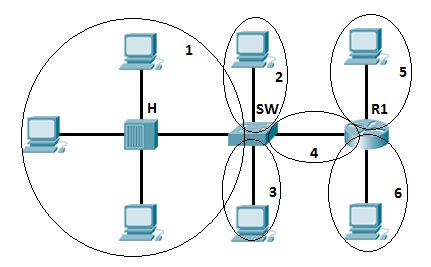
\includegraphics[scale=0.8]{pictures/CollisionDomains.jpg}
\end{figure}

\paragraph{Broadcast domain}is a domain in which a broadcast is forwarded. A broadcast domain contains all devices that can reach each other at the data link layer (OSI layer 2) by using broadcast. All ports on a hub or a switch are by default in the same broadcast domain. All hosts in the a VLAN are in the same broadcast domain regardless connecting to different switches. Every port on a router locates in a separate broadcast domain. Note that routers don't forward broadcasts from one broadcast domain to another.


\subsection{Memory Buffering on Switches}

There are two methods of memory buffering: Port-based Memory Buffering and Shared Memory Buffering.

\paragraph{Port-based Memory Buffering:} Frames are stored in queues that are linked to specific incoming and outgoing ports. A frame is transmitted to the outgoing port only when all the frames ahead of it in the queue have been successfully transmitted. 

\paragraph{Shared Memory Buffering:} deposits all frames into a common memory buffer that all the ports on the switch share.  The frames in the buffer are linked dynamically to the destination port. This allows the packet to be transmitted on a port without order and waiting. This method permits larger frames to be transmitted with fewer dropped frames. 

\section{Recovering from system crash}

The boot loader command line supports commands to format the flash file system, reinstall the operating system software, recover from system crash, recover a forgotten password. The boot loader command line can be accessed through a console connection following these steps:

\begin{enumerate}
\item Connect a PC by console cable to the switch console port. Configure terminal emulation software to connect to the switch.

\item Power off the switch by unplugging the switch power cord.

\item Reconnect the power cord to the switch and, within 15 seconds, press and hold down the Mode button while the System LED until it turns briefly amber and then solid green.
\end{enumerate}

\section{Configuration}

\subsection{Basic switch management}

To prepare a switch for remote management, it must be configured with an SVI, IP address, a subnet mask, and a default gateway. This is similar to configuring the IP address information on host devices. Please note that these IP settings are only for remote management access to the switch. The IP settings do not allow the switch to route Layer 3 packets.

\begin{sexylisting}{Basic switch management}
interface vlan 99
  ip address 172.17.99.11 255.255.255.0
  no shutdown
  exit
ip default-gateway 172.17.99.1
\end{sexylisting}

\subsection{Duplex configuration}

When a switch port is operating in full-duplex mode, there is no collision domain associated with the port. In contrast, half-duplex creates collision domain. The following command manually sets the F0/1 to full duplex and 100 Mb/s.

\begin{sexylisting}{Duplex configuration}
interface fa 0/1
  duplex full
  speed 100
  end
show interface
\end{sexylisting}

\subsection{Auto-MDIX}

When auto-MDIX is enabled, the interface automatically detects the required cable connection type (straight-through or crossover) and configures the connection appropriately. In other words, with auto-MDIX enabled, either type of cable can be used to connect to other devices.

\begin{sexylisting}{Auto-MDIX}
interface fastethernet 0/2
  mdix auto
  end
show controllers ethernet-controller fa 0/2 phy | include Auto-MDIX  
\end{sexylisting}

\subsection{SSH}

Before configuring SSH, the switch must be minimally configured with a unique hostname and the correct network connectivity settings. To display the version and configuration data for SSH on the device that you configured as an SSH server, use the \code{show ip ssh} command. To check the SSH connections to the device, use the \code{show ssh} command.

\begin{sexylisting}{SSH configuration}
ip domain-name cisco.com
ip ssh version 2
crypto key generate rsa
username admin secret ccna

line vty 0 15
  transport input ssh
  login local
end

show ip ssh
show ssh  
\end{sexylisting}

\subsection{Port security}

One way to secure ports is by implementing a feature called \emph{port security}. Port-security limits the number of valid MAC addresses allowed on a port. The MAC addresses of legitimate devices are allowed access, whereas other MAC addresses are denied. If a port is configured as a secure port and the maximum number of MAC addresses is reached, any additional attempts to connect by unknown MAC addresses generate a security violation.\\

Enable port-security feature will not work until the \code{switchport port-security} interface configuration command is executed. The type of secure address is based on the configuration and includes the following:

\begin{itemize}
\item \textbf{Static secure MAC addresses} are manually configured on a port. They are stored in the address table and are added to the running configuration on the switch.

%\begin{verbatim}
%S1(config)# interface f0/1
%S1(config-if)# switchport port-security mac-address aaaa.cafe.bbbb
%\end{verbatim}

\item \textbf{Dynamic secure MAC addresses} are dynamically learned and stored only in the address table. They are removed when the switch restarts.

\item \textbf{Sticky secure MAC addresses} can be dynamically learned or manually configured, and then stored in the address table and added to the running configuration. When sticky learning is enabled, the switch converts all dynamically learned MAC addresses, including those that were dynamically learned before sticky learning was enabled, into sticky secure MAC addresses. If sticky learning is disabled, the sticky secure MAC addresses remain part of the address table but are removed from the running configuration.

%\begin{verbatim}
%S1(config)# interface f0/1
%S1(config-if)# switchport port-security mac-address sticky
%\end{verbatim}
\end{itemize}

An interface can be configured for one of three violation modes: Protected, Restricted, and Shutdown. In these modes, a switch drops all frames with unknown source addresses until a sufficient number of these MAC addresses are removed, or the number of maximum allowable addresses is increased. No error messages are displayed in these modes.\\

\tableStart[\caption{Security violation mode}\label{Violation}] {| p{3cm} | p{3cm} | p{3cm} | p{3cm} |}
\head{Violation mode} & \head{Syslog message} & \head{Increase violation counter} & \head{Shut down port}\w
Protected & & & \w
Restricted & * & * & \w
Shutdown & & * & *\w
\tableEnd

%To change the violation mode on a switch port, use the following command:
%
%\begin{verbatim}
%S1(config)# interface f0/1
%S1(config-if)# switchport port-security violation protect
%S1(config-if)# switchport port-security violation restrict
%S1(config-if)# switchport port-security violation shutdown
%\end{verbatim}

\begin{sexylisting}{Port security configuration}
int f0/1
  switchport port-security
  switchport port-security mac-address sticky
  switchport port-security violation restrict
  switchport port-security maximum 2
end
show int  
show port-security int
\end{sexylisting}

\textbf{Shutdown} is the default violation mode. A port-security violation in this mode causes the interface to become \emph{error-disabled}. You can bring an error-disabled interface back to normal by entering \code{shutdown} followed by \code{no shutdown} command. When a port is error-disabled, the port LED will turn off, and the \code{show interface} command identifies the port status as \verb|err-disabled|. The output of the \code{show port-security int} command shows the port status as \verb|secure-shutdown|.\\

\textbf{Restrict} is the only port security mode that can assist with troubleshooting by sending syslog messages and keeping count of violations.

\section{Troubleshooting}

\subsection{Gathering symptoms}

The output from the \code{show int} command can be used to detect common media issues.

\begin{verbatim}
S1# show int f0/1
FastEthernet0/1 is up, line protocol is up (connected)
Hardware is Lance, address is 0022.91c4.0e01 (bia 0022.91c4.0e01)
MTU 1500 bytes, BW 100000 Kbit/sec, DLY 100 usec,
<output omitted>
\end{verbatim}

\begin{itemize}
\item The first parameter (\verb|FastEthernet0/1 is up|) refers to the \emph{physical layer} and indicates whether the interface is receiving a carrier detect signal. The second parameter (\verb|line protocol is up|) refers to the \emph{data link layer} and indicates whether the data link layer protocol keepalives are being received.

\item If the interface is up and the line protocol is down, there could be an \emph{encapsulation} type mismatch, or the interface on the other end could be \emph{error-disabled}.

\item If the line protocol and the interface are both down, a cable is not attached, or the other end of the connection may be administratively down.

\item If the interface is administratively down, it has been manually disabled (the \verb|shutdown| command has been issued) in the active configuration.
\end{itemize}

\begin{verbatim}
S1# show interfaces FastEthernet 0/1
FastEthernet0/1 is up, line protocol is up (connected)
<output omitted>

3 input errors, 3 CRC, 0 frame, 0 overrun, 0 ignored
0 watchdog, 120 multicast, 0 pause input
0 input packets with dribble condition detected
3594664 packets output, 436549843 bytes, 0 underruns
<output omitted>
\end{verbatim}

\textbf{Input errors} is the sum of all errors in frames that were received on the interface being examined. The reported input errors from the above output include the following:

\begin{itemize}
\item \textbf{Runt frames:} Ethernet frames that are shorter than the 64-byte (minimum allowed length of a frame) are called runt frames. Runt frames are caused by malfunctioning NIC or collisions.

\item \textbf{Giant:} Ethernet frames that are larger than 1518-byte (maximum allowed size of a frame) are called giants.

\item \textbf{CRC errors:} Common causes come from the cable (electrical interference, loose or damaged connections, and incorrect cabling). If you see many CRC errors, there is too much noise on the cable and you should inspect the cable. You should also search for and eliminate noise sources.
\end{itemize}

\begin{verbatim}
S1# show interfaces FastEthernet 0/1
FastEthernet0/1 is up, line protocol is up (connected)
<output omitted>

8 output errors, 1790 collisions, 10 interface resets
0 unknown protocol drops
0 babbles, 235 late collision, 0 deferred
0 lost carrier, 0 no carrier, 0 pause output
0 output buffer failures, 0 output buffers swapped out
\end{verbatim}

\textbf{Output errors} is the sum of all errors that prevented the final transmission of frames out the interface that is being examined. The reported output errors include the following:

\begin{itemize}
\item \textbf{Collisions:} Collisions in half-duplex operations are normal. However, you should never see collisions on an interface configured for full-duplex communication.

\item \textbf{Late collision:} A late collision refers to a collision that occurs after \textbf{512 bits} of the frame have been transmitted. Common causes: Excessive cable lengths, Duplex mismatch.
\end{itemize}

\subsection{Take action}

If the interface is down, take these two actions:

\begin{enumerate}
\item Check the \emph{cable}. Make sure the proper and non-damaged cables are being used.

\item If the interface is still down, the problem may be due to a \emph{speed mismatch}. Manually set the same speed on both connection ends if this problem is suspected.
\end{enumerate}

If the interface is up, but issues with connectivity are still present, do the following:

\begin{enumerate}
\item Using the \verb|show interfaces| command, check for indications of excessive \emph{noise}. Indications may include an increase in the counters for runts, giants, and CRC errors. If there is excessive noise, find and remove the source of the noise, verify that the cable does not exceed the maximum cable length and check the cable type.

\item If noise is not an issue, check for excessive \emph{collisions}. If there are collisions or late collisions, the problem may be due to \emph{duplex mismatch}. If this is true, manually set the duplex to full on both ends of the connection.
\end{enumerate}